\section{Related Work}
\label{sec:related}

% Method overview: placed here so that it floats to the top of page 3 as Fig. 2.
% Fig. 2: research/paper/figures/fig2_method.py writes figures/figure2_laq_editable.pptx; figures/figure2.pdf is its vector export from PowerPoint.
\begin{figure*}[t]
  \centering
  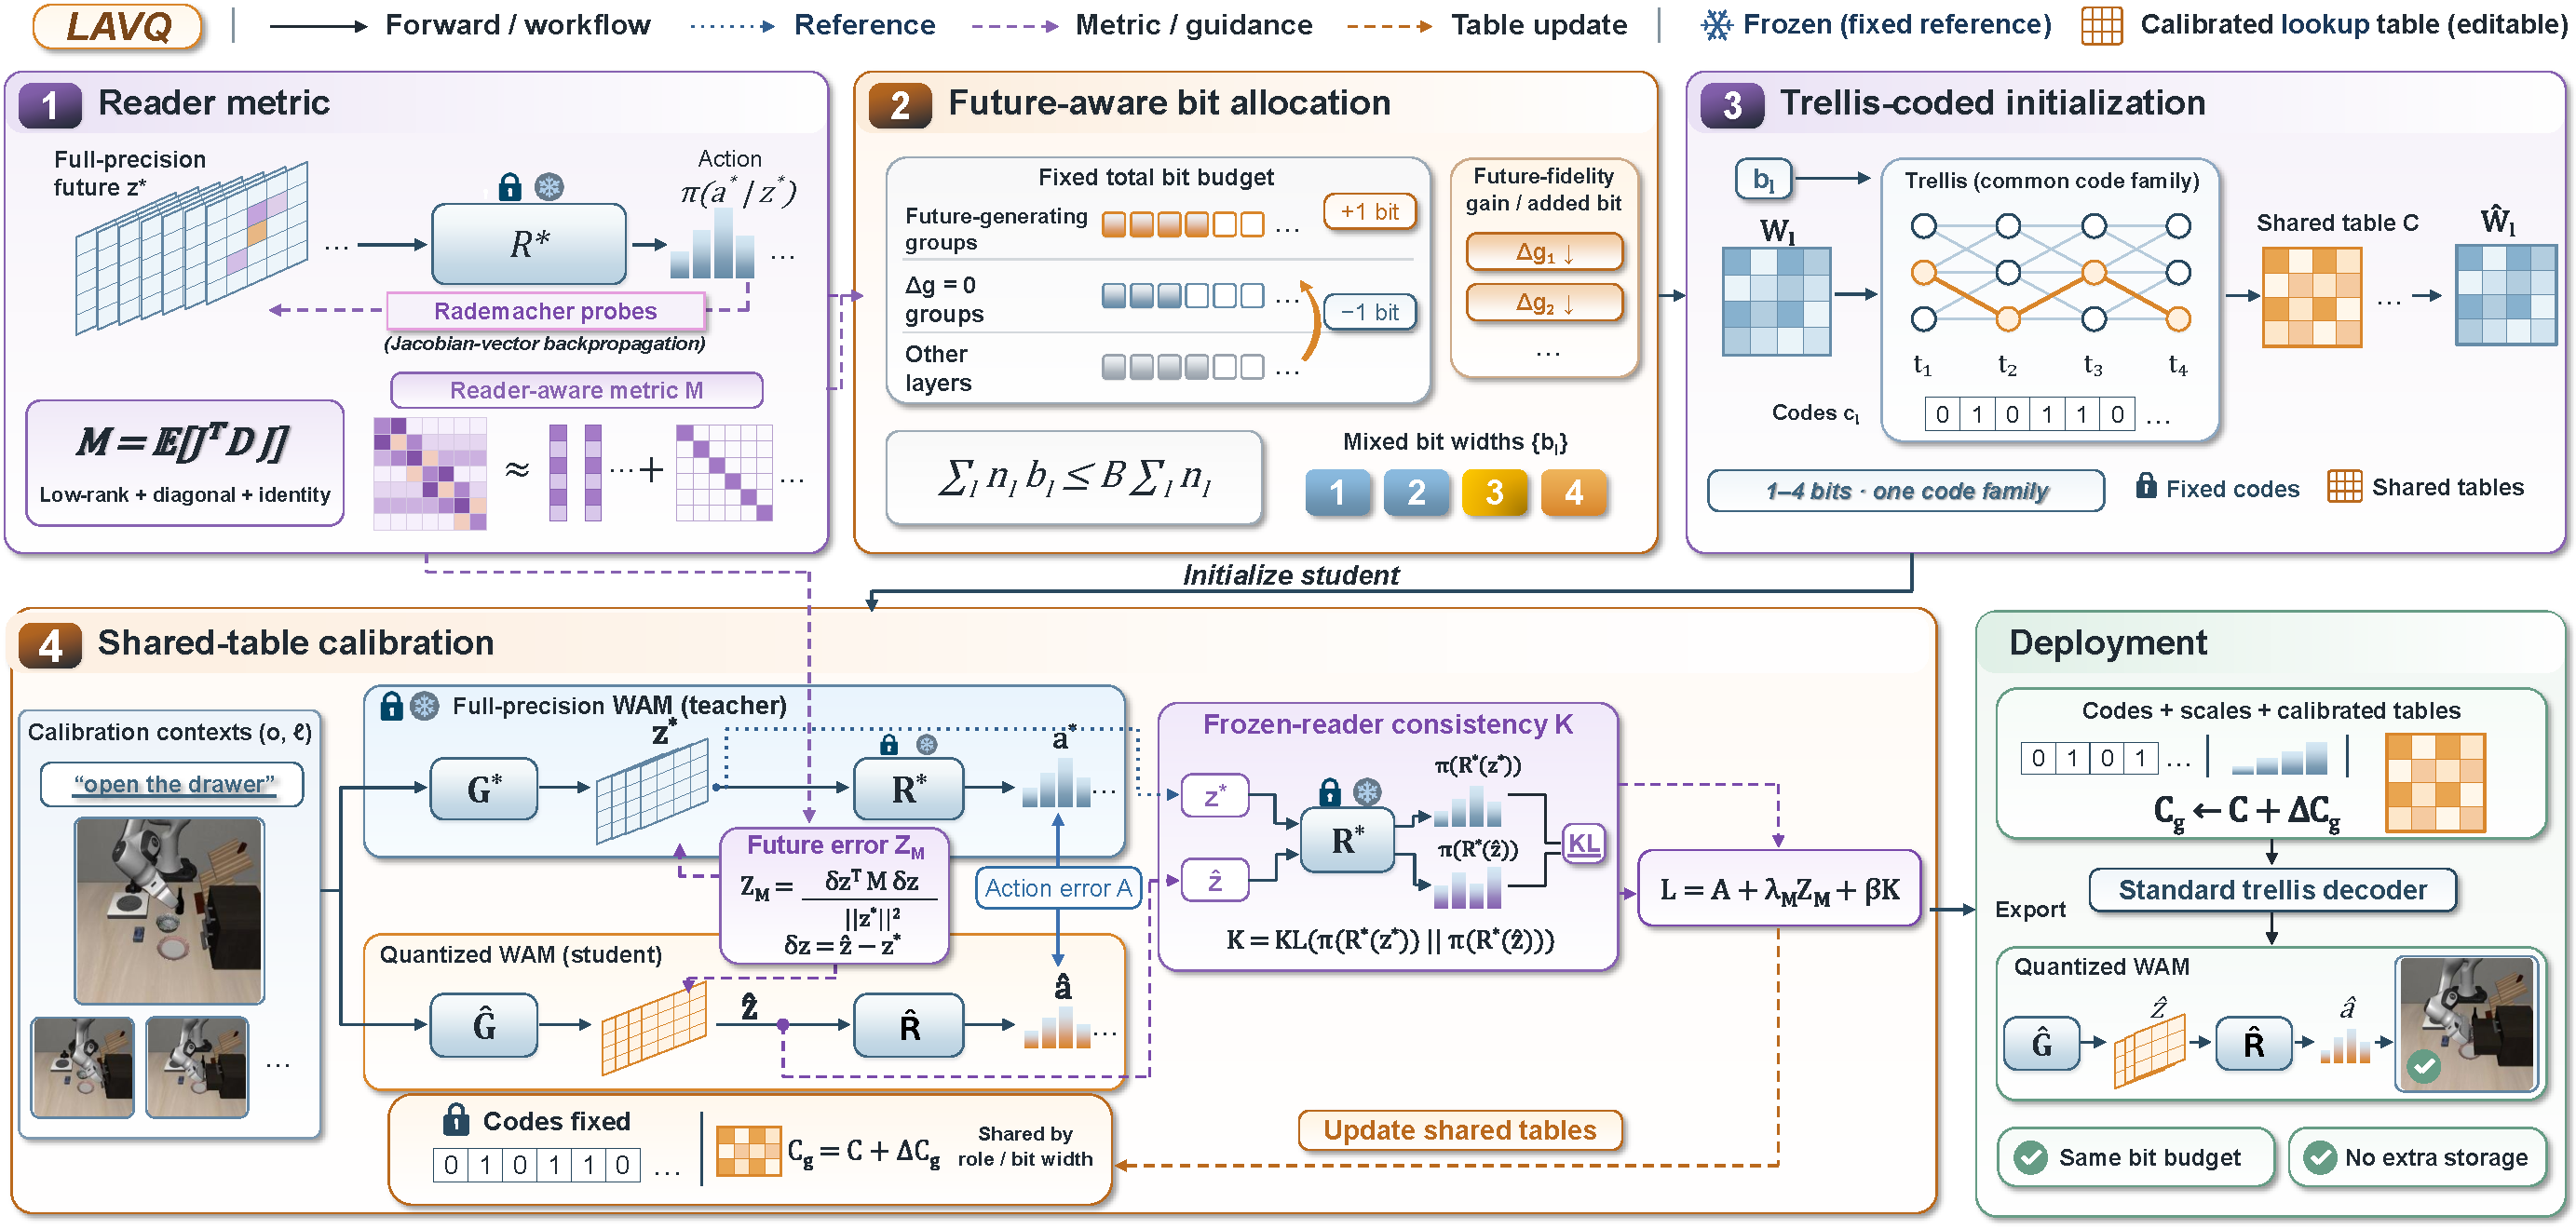
\includegraphics[width=\textwidth]{figures/figure2.pdf}
  \caption{Overview of \method.
  Offline, \method estimates the reader metric $\bM$, which measures future error as the reader sees it~(a), measures the read count $n_u$, the damage of a rounding error that is frozen across the denoising steps relative to one that is redrawn at every step~(b), and solves one objective for the 4-bit weights and for a threshold $\mu$ shared by activations and caches~(c).
  At every control step, gaze-guided refinement~(d) scores the tokens under the current gaze, quantizes the residual of the selected tokens with a second 4-bit code, and applies both codes in the linear layers and in the cache; the attention of the action tokens gives the gaze for the next step.
  Every weight stays at 4 bits.}
  \label{fig:method}
\end{figure*}

\paragraph{World action models.}
World action models train a video generator jointly with an action model, so that actions are conditioned on a predicted future~\cite{yuan2026fastwam,kim2026cosmospolicy,li2026lingbotva,ye2026dreamzero}.
They extend vision-language-action policies~\cite{kim2024openvla,black2024pi0} with the visual priors of video backbones and inherit their size.
We do not modify how WAMs are trained and study only how to compress them for deployment.

\paragraph{Post-training quantization.}
Second-order rounding quantizes one layer at a time and compensates the error with the inverse Hessian of a layer-wise reconstruction objective~\cite{frantar2022obc,frantar2023gptq}.
Activation-aware scaling~\cite{xiao2023smoothquant,lin2024awq} and rotations~\cite{ashkboos2024quarot,liu2025spinquant,chen2026prismquant} remove activation outliers before rounding and bring language models to 4-bit weights, activations and key--value caches.
Mixed-precision methods allocate bit widths across layers~\cite{wang2019haq,malinovskii2025higgs}, and GuidedQuant weights the layer objective with gradients of the end loss~\cite{kim2025guidedquant}.
For diffusion and video generators, post-training methods correct errors that accumulate over the denoising loop~\cite{he2023ptqd}, handle timestep-dependent activations~\cite{zhao2025viditq} and absorb outliers into a 16-bit low-rank branch~\cite{li2025svdquant}, and quantization-aware training reaches 4 bits and below~\cite{huang2026qvgen,li2026dsaquant}.
For vision-language models, GRACE combines quantization-aware training with confidence-gated distillation to reach 4 bits~\cite{chen2026grace}.
These methods preserve layer outputs or generation quality.
\method builds on rotation and second-order rounding, and changes what the quantizer preserves: the predicted future as the reader sees it.

\paragraph{Quantization of robot policies and WAMs.}
For vision-language-action models, QuantVLA and BitVLA compress the policy with calibrated scales and 1-bit weights~\cite{zhang2026quantvla,wang2025bitvla}.
For WAMs, QuantWAMs calibrates protection decisions for channels, layers and denoising steps at the right granularity~\cite{zhou2026quantwams}, Q-WAM selects the activation subspace that drives the final action through the unrolled sampler and keeps it in a 16-bit branch~\cite{akbari2026qwam}, and SteerQuant routes errors across token streams and denoising steps by their impact on the action~\cite{wang2026steerquant}.
PreDE predicts the task degradation of a quantization configuration from offline action deviations~\cite{xu2026prede}.
These quantizers measure sensitivity with respect to the final action or the training loss, one denoising step at a time.
\method instead targets the predicted future that the action is read from, counts how often each rounding error is read, and extends quantization to the caches.

\paragraph{Token-level precision.}
Several quantizers spend more bits on a few tokens.
Squat keeps the tokens with the highest attention at 8 bits and the rest at 4~\cite{shen2024squat}, STaMP transforms activations along the sequence so that a few tokens carry most of the energy and receive higher precision~\cite{federici2026stamp}, SemanticDialect re-quantizes the residual of salient tokens in video diffusion transformers~\cite{jang2026semanticdialect}, and ZipCache assigns cache precision by token saliency~\cite{he2024zipcache}.
In all of them, a model's own attention or activation energy decides which tokens matter.
In a WAM, the predicted future is consumed by a different part of the model, and \method lets this reader decide: tokens are selected by their effect on the action, and tracked at run time through the attention of the action tokens.
